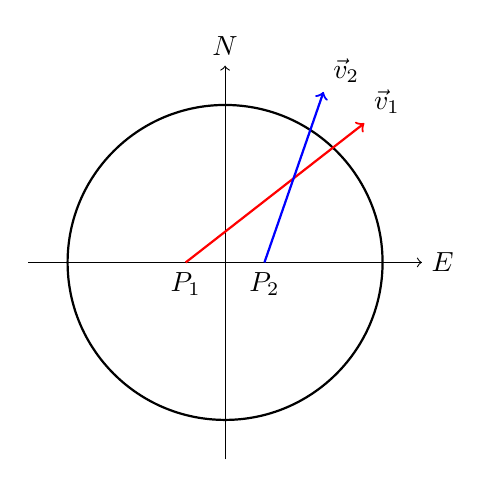
\begin{tikzpicture}
	% Draw the circle
	\draw[thick] (0,0) circle (2cm);
	
	\pgfmathsetmacro{\angB}{45} 
	\pgfmathsetmacro{\angA}{30} 
	\pgfmathsetmacro{\R}{2.5} 

	% Draw the coordinate system
	\draw[->] (0,-\R) -- (0,\R) node[above] {$N$};
	\draw[->] (-\R,0) -- (\R,0) node[right] {$E$};
	
	% Define the angle alpha
%	\def\angB{45}
%	\def\angA{30}
%	\def\R{2.5}
	
	% Draw the vectors
	\draw[->, thick, red] (-0.5,0) -- ({\R*sin(\angB)}, {\R*cos(\angB)}); % node[midway, above right] {$\vec{v}_1$};
	\draw[->, thick, blue] (0.5,0) -- ({\R*sin(\angA)}, {\R*cos(\angA)}); %node[midway, above left] {$\vec{v}_2$};
	
	% Draw the angle alpha
	%\draw[thick] (1.3,0) arc[start angle=0, end angle =\angB, radius=0.5];
%	\node at ({1.2+0.7*sin(\angB/2)}, {-0.4 + 0.7*cos(\angB/2)}) {$\alpha_2$};
	
	% Draw the angle alpha on the opposite side
	%\draw[thick] (-0.5,0) arc (0:\angA:0.5);
%	\node at ({-0.7*sin(\angA/2)}, {-0.4 + 0.7*cos(\angA/2)}) {$\alpha_1$};
	
	% Label the points
	\node at ({\R*sin(\angB)}, {\R*cos(\angB)}) [above right] {$\vec{v}_1$};
	\node at ({\R*sin(\angA)}, {\R*cos(\angA)}) [above right] {$\vec{v}_2$};

	% Label the points
	\node at ({-0.5}, {0}) [below] {$P_1$};
	\node at ({ 0.5}, {0}) [below] {$P_2$};
\end{tikzpicture}


